%template1.tex
%The following LaTeX source file represents the simplest kind of slide presentation; no overlays, no included graphics. Substitute your favorite style for ``pascal''. To create the PDF file template1.pdf, (1) be sure to use the prosper class, then (2) execute the command latex template1.tex, and (3) the command dvipdf template1.dvi.

%%%%%%%%%%%%%%%%%%%%%%%%%%%%%%% template1.tex %%%%%%%%%%%%%%%%%%%%%%%%%%%%%%%%%%%
\documentclass[a4paper,blends,pdf,colorBG,slideColor]{prosper}
% definitions for slides for CSC544
% Lutz Hamel, (c) 2007

\hypersetup{pdfpagemode=FullScreen}

\usepackage{times}
\usepackage{latexsym}
\usepackage{alltt}
\usepackage{booktabs}
\usepackage{amsmath}
\usepackage{amsopn}
\usepackage{amsfonts}
\usepackage{amssymb}
%\usepackage[usenames]{color}

\def\sign{\qopname\relax{no}{sign}}
\def\argmax{\qopname\relax{no}{argmax}}
\def\argmin{\qopname\relax{no}{argmin}}

\newcommand{\grad}{\ensuremath{\nabla}} 
\newcommand{\loss}{\ensuremath{{\cal L}}}
\newcommand{\err}{\mbox{err}}
\newcommand{\mse}{\mbox{mse}}
\newcommand{\acc}{\mbox{acc}}
\newcommand{\Integer}{\ensuremath{\mathbb{N}}}
\newcommand{\size}[1]{{|{#1}|}}
\newcommand{\Rnspace}[1]{\ensuremath{\mathbb{R}^{#1}}}
\newcommand{\Real}{\ensuremath{\mathbb{R}}}
\newcommand{\mytt}[1]{{\small\tt{#1}}}
\newcommand{\textemph}[1]{{\em #1}}
\newcommand{\suchthat}{\mid}
\newcommand{\orbar}{\;|\;}
\newcommand{\bs}[1]{\begin{slide}{#1}\ptsize{8}}
\newcommand{\es}{\end{slide}}
\newcommand{\co}{\,\colon\;}
\newcommand{\pair}[2]{\ensuremath{( {#1}, {#2} )}}
\newcommand{\model}[1]{\hat{#1}}
\newcommand{\ul}[1]{{\bf\em #1}}
\newcommand{\ol}{\overline}
\newcommand{\definition}[1]{{\bf Definition: }{\em #1}}
\newcommand{\example}[1]{{\bf Example: }{#1}}
\newcommand{\abs}[1]{|{#1}|}
\newcommand{\mytab}{\makebox[.1in]{}}

\newcommand{\fdef}[1]{
\begin{center}
\fbox{
\begin{minipage}{3.5in}
{\bf Definition:}
{#1}
\end{minipage}
}
\end{center}
}

\newcommand{\fframe}[1]{
\begin{center}
\fbox{
\begin{minipage}{3.5in}
{#1}
\end{minipage}
}
\end{center}
}

\newcommand{\nframe}[1]{
\begin{center}
\begin{minipage}{3.5in}
{#1}
\end{minipage}
\end{center}
}

\newenvironment{Rcode}
	{
		\scriptsize
		\begin{quote}
		\begin{alltt}
	}
	{
		\end{alltt}
		\end{quote}
	}




\begin{document}

\bs{Novelty Dectection}
\small
Novelty/outlier detection -- find points in an {\em unlabeled} data set that do not
conform to the general distribution pattern of the overall data set.

The central idea in novelty detection with maximum margin machines is to construct
a hyperplane through the origin of the input space whose margin separates the unlabeled training points  from the origin in some optimal way.
\begin{center}
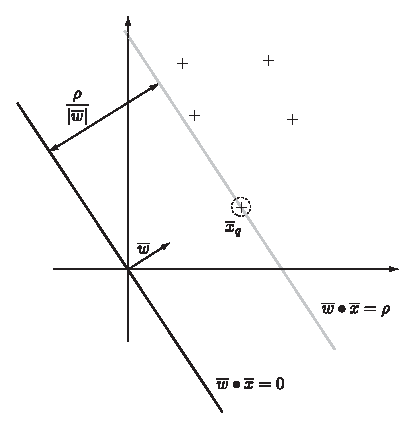
\includegraphics[height=40mm]{figures/fig13-01.eps}
\end{center}
\es

\bs{Maximum Margin Machines}
Assume we have an unlabeled training set,
\begin{equation*}
D = \{ \ol{x}_1, \ol{x}_2,\ldots,\ol{x}_l \} \subset \Rnspace{n}.
\end{equation*}
whose elements are located only in the first hyperoctant (the components of all vectors are positive) and can be linearly separated from the origin.

In this case maximizing the margin of a hyperplane going through the origin
gives rise to the following convex optimization
problem,
\begin{align*}
\min \phi(\ol{w},\rho) = \min_{\ol{w},\rho} \frac{1}{2} \ol{w}\bullet\ol{w} - \rho,\\
\intertext{subject to the constraints,}
 \ol{w}\bullet\ol{x}_i \ge \rho,
\end{align*}
where $\ol{x}_i \in D$.

\es

\bs{Outliers are Margin Errors!}
\small
\begin{center}
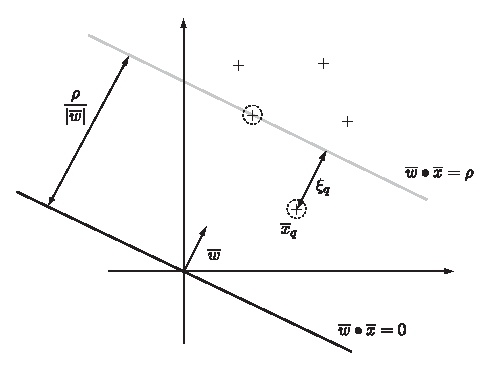
\includegraphics[height=35mm]{figures/fig13-02.eps}
\end{center}

\begin{equation*}
\min \phi(\ol{w},\rho) = \min_{\ol{w},\rho} \frac{1}{2} \ol{w}\bullet\ol{w} - \rho + {\color{red}\frac{1}{\nu\, l}}\sum_{i = 1}^l \xi_i,
\end{equation*}
subject to the constraints,
\begin{align*}
\ol{w}\bullet\ol{x}_i &\ge \rho - \xi_i,\\
\xi_i &\ge 0,
\end{align*}
for $i = 1,\ldots,l$ and $0 < \nu \le 1$. 
\es

\bs{Classifying Outliers}
We can perform a simple trick  that allows us to construct a decision surface that will classify any point not in the training data
as a novelty or not:  
\begin{quote}
\em We translate the hyperplane that runs
through the origin in such a way that it coincides with the supporting hyperplane of the margin and
consider it a decision surface that separates outliers from the rest of the data.
\end{quote}
More formally,
\begin{equation*}
\model{f}(\ol{x}) = \ol{w}^*\bullet\ol{x} - \rho^*,
\end{equation*}
where $\ol{w}^*$ and $\rho^*$ are solutions to the Lagrangian dual.

Now, given a point $\ol{z}\in \Rnspace{n}$, if that point lies below the decision surface, $\model{f}(\ol{z}) < 0$, then we consider the point an outlier.

\es


\bs{The Dual}
\small
For the dual we construct the Lagrangian,
\begin{equation*}
\begin{aligned}
L(\ol{\alpha},\ol{\beta},\ol{w},\rho,\ol{\xi}) &=\frac{1}{2} \ol{w}\bullet\ol{w} - \rho + \frac{1}{\nu\, l}\sum_{i = 1}^l \xi_i\\
&\quad - \sum_{i=1}^l \alpha_i\left(\ol{w}\bullet\ol{x}_i - \rho + \xi_i\right)\\
&\quad - \sum_{i=1}^l \beta_i\xi_i.
\end{aligned}
\end{equation*}

As usual we formulate this as the Lagrangian optimization,
\begin{equation*}
\max_{\ol{\alpha},\ol{\beta}} \min_{\ol{w},\rho,\ol{\xi}} L(\ol{\alpha},\ol{\beta},\ol{w},\rho,\ol{\xi}),
\end{equation*}
subject to the constraints,
\begin{align*}
\alpha_i &\ge 0,\\
\beta_i &\ge 0,
\end{align*}
for $i = 1,\ldots,l$. 
\es

\bs{The Dual}
It is now straightforward to state the KKT conditions and from a solution that has to satisfy the
KTT conditions it is easy to derive the dual,
\begin{equation*}
\max \phi'(\ol{\alpha}) = \max_{\ol{\alpha}}\left ( - \frac{1}{2} \sum_{i=1}^l \sum_{j=1}^l \alpha_i \alpha_j \ol{x}_i\bullet\ol{x}_j \right ),
\end{equation*}
subject to the constraints,
\begin{align*}
\frac{1}{\nu\,l} \ge \alpha_i &\ge 0,\\
\sum_{i=1}^l \alpha_i & = 1,
\end{align*}
for $i = 1,\ldots,l$.

\es

\bs{Novelty Detection in R}
\begin{Rcode}
library(e1071)
# setup our output device
quartz(height=4,width=4,pointsize=8)

# create a 2D data set and plot as squares
x1 <- rnorm(10,mean=4)
x2 <- rnorm(10,mean=4)
x <- data.frame(x1,x2)
plot(x,pch=22,cex=.5,xlim=c(-2,8),ylim=c(-2,8))

# build the novelty detection model
model <- svm(x,
             type="one-classification", 
             kernel="linear",
             nu=0.1,
             scale=FALSE)

# plot the support vector outliers as filled squares
ix <- model$index[model$coefs == 1.0]
x1 <- x$x1[ix]
x2 <- x$x2[ix]
sv <- data.frame(x1,x2)
points(sv,type="p",pch=22,cex=.5,bg="red",col=2)
\end{Rcode}
\es

\bs{Novelty Detection in R}
\begin{Rcode}
# plot the hyperplane together with the 
# margin that constitutes the novelty decision surface
w1 <- sum(x$x1[model$index]*model$coefs)
w2 <- sum(x$x2[model$index]*model$coefs)
slope <- -(w1/w2)
offset <- (model$rho/w2)
abline(a=offset,b=slope,lty=2)
abline(a=0,b=slope)
\end{Rcode}

\begin{center}
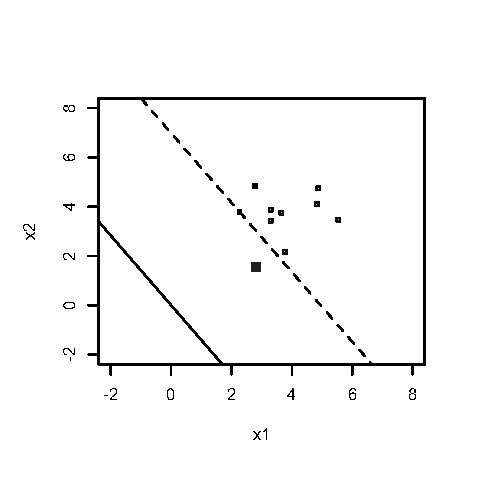
\includegraphics[height=45mm]{figures/fig13-03.eps}
\end{center}

\es

\bs{Novelty Detection in R}

\begin{Rcode}
library(e1071)
# setup our output device
quartz(height=4,width=4,pointsize=8)

# create a 2D data set and plot as squares
x1 <- rnorm(100)
x2 <- rnorm(100)
x <- data.frame(x1,x2)
plot(x,pch=22,cex=.5,xlim=c(-4,4),ylim=c(-4,4))

# build the novelty detection model
model <- svm(x,
             type="one-classification",
             kernel="radial",
             gamma=0.1,
             nu=0.05)

# plot the support vectors as filled squares
ix <- model$index[model$coefs == 1.0]
x1 <- x$x1[ix]
x2 <- x$x2[ix]
sv <- data.frame(x1,x2)
points(sv,type="p",pch=22,cex=.5,bg="red",col=2)
\end{Rcode}
\es

\bs{Novelty Detection in R}

\begin{center}
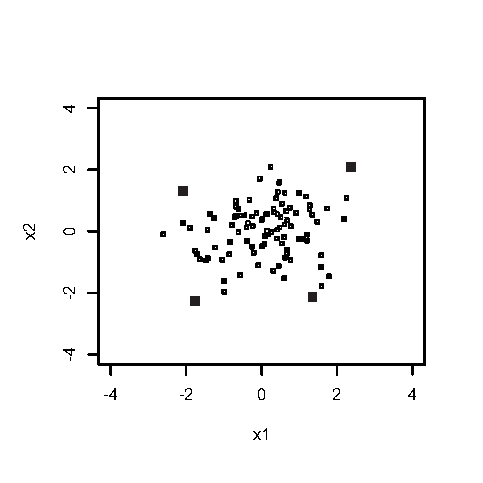
\includegraphics[height=50mm]{figures/fig13-04.eps}
\end{center}
\es

\end{document}
%%%%%%%%%%%%%%%%%%%%%%%%%%% end of template1.tex %%%%%%%%%%%%%%%%%%%%%%%%%%%%%%%%

